\documentclass[journal,12pt,twocolumn]{IEEEtran}
\usepackage[none]{hyphenat}
\usepackage{enumitem}
\usepackage{graphicx}
\usepackage{listings}
\usepackage{kvmap}
\usepackage[utf8]{inputenc}
\usepackage{caption}
\usepackage{url}
\usepackage{hyperref}


\title{Assignment \textrm{I} \\ \textbf{\\JOHNSON COUNTER}}
\author{Manoj Chavva- FWC22055}

\begin{document}
\maketitle

\tableofcontents
\vspace{0.5cm}
\begin{abstract}
  This Manual shows the design and Implemantation of four bit Johnson counter.
\end{abstract}   


 
     \section{Components}  
       

\begin{tabular}{|c|c|c|}
    \hline 
      \textbf{S.No} & \textbf{Component} & \textbf{Number}\\
      \hline
	1. & Arduino & 1 \\
	2. & Bread Board & 1 \\
	3. & Jumper Wires(M-M) & 6 \\
	4. & LED & 4 \\
	
      \hline
      
   \end{tabular}
   

     \vspace{0.35cm}




\section{Introduction}
\begin{enumerate}
  \item Johnson counters are used to store or process or count the number of events occurred within the circuit.
  \item It is designed with a group of flip-flops, where the inverted output from the last flip-flop is connected to the input of the first flip-flop.
  \item In Johnson counter
  \\No. of states = No. of flip-flop used  
\\Number of used states=2n  
\\Number of unused states=2n - 2*n  
\item Here, the functionality of D flip flop is used for the program. 
\end{enumerate}

    \vspace{2.5cm}   



\section{Circuit Diagram}
\begin{enumerate}
\item The inverted output of the last flip-flop ‘$\bar{Q}$n’ is fed back to the first flip-flop in the sequence bit pattern. 
\item The counter registers cycles in a closed-loop i.e circulates within the circuit.
\begin{figure}[h]
    \centering
    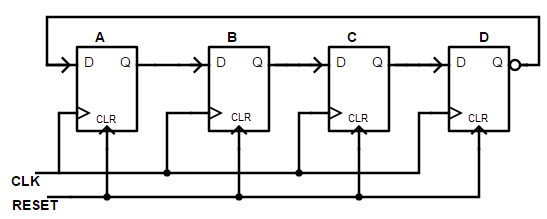
\includegraphics[width=8cm, height=4.2cm]{counter.jpg}
    
    \caption{Four bit Johnson Counter}

\end{figure}
\item Reset pin acts as an on/off switch. So, the flip-flops can be enabled by clicking the Reset switch.

\item CLK pin is used to observe the changes in the output of the flip-flops.
\end{enumerate}



\section{Procedure}
\begin{enumerate}
\item Connect the 4 LED's and Aurdino according to table \ref{table:1}
\item Observe the states of LED and verify the truth table using the code from the link.



\end{enumerate}

\begin{table}[h]
\centering
\large
\begin{tabular}{|l|l|l|l|l|l|}
\hline
\textbf{Arduino} & D2   & D3   & D4   & D5   & GND \\ \hline
\textbf{LED's}   & LED1 & LED2 & LED3 & LED4 &     \\ \hline
\end{tabular}
\caption{Connection Table}
\label{table:1}
\end{table} 

\newpage

\begin{table}[h]
\large
\centering
\begin{tabular}{|l|}
\hline

\url{https://github.com/ManojChavva/FWC/blob/main/Assignement1/JohnsonWithoutIC/code.cpp} \\
\hline

\end{tabular}

\end{table}





\section{Truth Table}



\begin{center}
    
    \setlength{\arrayrulewidth}{0.5mm}
\setlength{\tabcolsep}{18pt}
\renewcommand{\arraystretch}{1.5}
    \begin{tabular}{|l|c|r|l|c|}
    \hline 
      \textbf{state} & \textbf{$ Q_{0} $} & \textbf{$ Q_{1} $} & \textbf{$ Q_{2} $} & \textbf{$ Q_{3} $}
      \\
      \hline
          0&0&0&0&0
          \\ 1&1&0&0&0
          \\ 2&1&1&0&0
          \\ 3&1&1&1&0
          \\ 4&1&1&1&1
          \\ 5&0&1&1&1
          \\ 6&0&0&1&1
          \\ 7&0&0&0&1 \\
      \hline
      
   \end{tabular}
   
   \vspace{0.5cm}
   \centering Table II: Truth Table.
\label{table:2}
 \end{center}
 \begin{itemize}
 \item The above table state that
 \end{itemize}
 \begin{enumerate}
 
\item The counter produces the output 0000 when there is no clock input passed(0).
\item  The counter produces the output 1000 when the 1st clock pulse is passed to the flip flops.
 \item  The counter produces the output 1100 when the 2nd clock pulse is  \item The counter produces the output 1110 when the 3rd clock pulse is passed to the flip flops.
\item The counter produces the output 1111 when the 4th clock pulse is  passed to the flip flops.
\item  The counter produces the output 0111 when the 5th clock pulse is passed to the flip flops.
\item The counter produces the output 0011 when the 6th clock pulse is passed to the flip flops.
\item The counter produces the output 0001 when the 7th clock pulse is passed to the flip flops.
 \end{enumerate}
 
 
 \section*{Conclusion}
 Thus the Johnson counter designed and Implemented.

\end{document}
